\documentclass[letterpaper]{article}
\usepackage{inconsolata}
\usepackage[T1]{fontenc}
\usepackage[margin=1in]{geometry}
\usepackage[utf8]{inputenc}
\usepackage{hyperref}
\usepackage{soul}
\usepackage{fancyhdr, lastpage}
\usepackage{graphicx}
\pagestyle{fancy}
\fancyhf{}
\usepackage{minted}
\usemintedstyle{pastie}

\newcommand{\spacer}{\vspace{5mm}\hrule\vspace{5mm}}

\makeatletter
\renewcommand{\@maketitle}{
  \begin{center}%
    {\LARGE \@title \par}%
  \end{center}%
  \vspace*{40pt}
  \noindent \Large \@date \par %
  \vspace*{20pt}
  \noindent \Large \@author \par %
  \vfill
  \par
}
\makeatother

% New commands
\newcommand{\assignmentnumber}{2-4}
\newcommand{\course}{CS 444: Compiler Construction}
\newcommand{\term}{Winter 2014}
\newcommand{\project}{Labs \assignmentnumber: Name Resolution, Type Checking, Static Analysis}
\newcommand{\name}{wlue, cktaylor, psobot}
\newcommand{\wenhao}{wlue(20349659) - Lue, Wen-Hao (wlue@uwaterloo.ca)}
\newcommand{\chris}{cktaylor(20338058) - Taylor, Chris (cktaylor@uwaterloo.ca)}
\newcommand{\peter}{psobot(20334978) - Sobot, Peter (psobot@uwaterloo.ca)}

% Values for template
\title{\course \\ \term \\ \project}
\date{\ul{\textbf{Date of Submission}}: \today}
\author{\ul{\textbf{Submitted by}}: \\ \indent \wenhao \\ \indent \chris \\ \indent \peter}

\rhead{\name{}}
\lhead{\course{} Assignment \assignmentnumber}
\cfoot{Page \thepage{} of \protect\pageref{LastPage}}

% Content
\begin{document}

  \maketitle
  \thispagestyle{empty}
  \clearpage

  \setcounter{page}{1}

  \clearpage
  \section{Introduction}

  Our Joos1W compiler, named {\em Joosbox}, currently performs the following
  operations on all programs passed in on the command line:

  \begin{itemize}
    \item Scanning
    \item Parsing
    \item Weeding
    \item Environment Building
    \item Type Linking
    \item Hierarchy Checking
    \item Name Resolution
    \item Type Checking
    \item Static Analysis
  \end{itemize}

  When passed a valid Joos1W program, Joosbox will print nothing on standard
  error or standard output, and will return a {\tt 0} return code. Upon
  parsing an invalid Joos1W program, Joosbox will output diagnostic
  information (including line number and character index of invalid tokens, if
  available) to the standard error stream. Joosbox will then return {\tt 42}.

  Joosbox is implemented in Scala, and makes use of only four libraries ---
  the Scala standard library, the {\tt SBT} built tool, the {\tt Specs2}
  testing framework, and Apache Commons Lang. This document outlines the
  design of Joosbox, enumerates the significant challenges encountered during
  its construction, and describes our group's testing process.

  \section{Design}

  Each major component of Joosbox is implemented as a separate Scala singleton
  object, with no state but numerous methods for traversing the Joos abstract
  syntax tree and performing operations on it. Joosbox's abstract syntax tree
  data types and construction methods did not change significantly from their
  original implementation in assignment 1, although numerous abstract syntax
  nodes were corrected or expanded to have additional methods useful for later
  stages of the program.

  In Scala, each abstract syntax node is implemented as a {\tt case class},
  with the constructor arguments to each node being its direct children.
  For instance, the following code describes the case class used for
  compilation units in a Joos program:

  \begin{verbatim}
case class CompilationUnit(
  packageDeclaration: Option[PackageDeclaration] = None,
  importDeclarations: Seq[ImportDeclaration] = Seq.empty[ImportDeclaration],
  typeDeclaration: Option[TypeDeclaration] = None
) extends AbstractSyntaxNode {
  override def children: List[AbstractSyntaxNode] =
    packageDeclaration.toList ++ importDeclarations.toList ++ typeDeclaration.toList
}
  \end{verbatim}

  Each case class member of this {\tt AbstractSyntaxNode} is explicit about
  its purpose and its type, which allows us to use Scala's powerful type
  system to manipulate and traverse the structure of each program without
  having to write overly verbose code.

  \subsection{Environment Building}

  To allow Joosbox to effectively manage the concept of scope while parsing
  Joos programs, we implemented an environment building step after our
  compiler creates an abstract syntax tree. This step, implemented as the {\tt
  EnvironmentBuilder} object, traverses the abstract syntax tree by means of a
  recursive Scala function. Each time a node is reached that could create a
  new scope, this function would match the node and create this scope,
  consisting of a mapping between a name and an abstract syntax node. New
  scopes were created for each  of the following node types:

  \begin{itemize}
    \item {\tt CompilationUnit}
    \item {\tt ClassDeclaration}
    \item {\tt MethodDeclaration}
    \item {\tt ConstructorDeclaration}
    \item {\tt FieldDeclaration} (and its initializer)
    \item {\tt Block}
    \item {\tt LocalVariableDeclaration}
  \end{itemize}

  Figure~\ref{fig:environments} shows a graphical illustration of the nested
  scopes created by Joosbox during this phase.

  \begin{figure}[h!]
    \caption{The nested scopes created by Joosbox's {\tt EnvironmentBuilder}.}
    \centering
    \begin{center}
      \makebox[\textwidth]{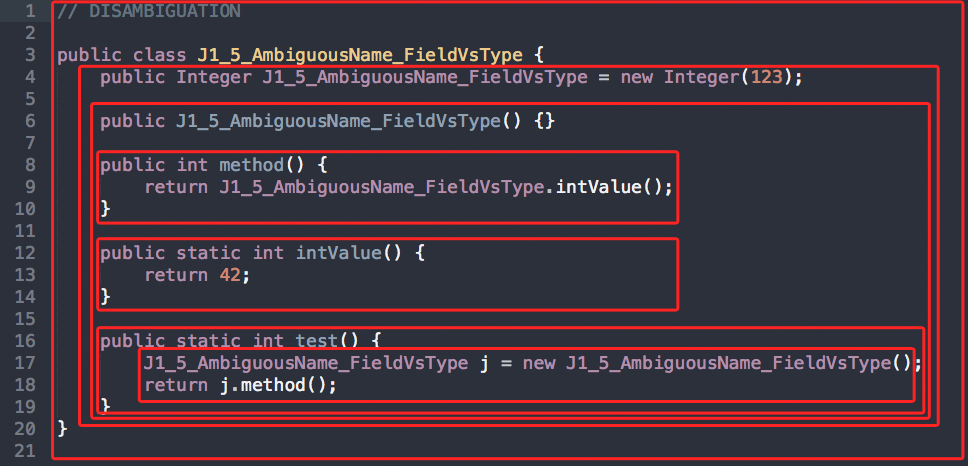
\includegraphics[width=\textwidth]{environments.png}}
    \end{center}
    \label{fig:environments}
  \end{figure}

  Once this recursive environment building step is complete, each node has its
  own local scope variable assigned to the scope that it resides in. By
  directly mapping nodes to their enclosing environment, performing checks to
  see what other nodes are ``in scope'' becomes simple. For instance, looking up
  an expression named {\tt foo} in the local scope can be as easy as:

  \begin{verbatim}
    node.scope.get.lookup(ExpressionNameLookup(ExpressionName("foo")))
    // -> returns an Option[AbstractSyntaxNode]
  \end{verbatim}

  This call to {\tt lookup} uses the hierarchical nature of the scope tree
  to bubble up each request all the way to the root node. If any expression
  named {\tt foo} is visible from the node's scope, then it will be returned ---
  however, types or methods named {\tt foo} will not. This separation of
  {\tt ExpressionName}, {\tt TypeName}, and so on was accomplished by
  encoding the type (expression, type, etc.) of each entry in each scope's mapping with
  Scala's type system. Each scope contains a map defined as such:

  \begin{verbatim}
    val locals: Map[EnvironmentLookup, Referenceable]
  \end{verbatim}

  In the above mapping, {\tt EnvironmentLookup} is a sealed Scala trait, not a concrete
  class, which means that every kind of lookup must be one of:

  \begin{itemize}
    \item {\tt TypeNameLookup}
    \item {\tt ExpressionNameLookup}
    \item {\tt MethodLookup}
    \item {\tt ConstructorLookup}
  \end{itemize}

  The use of a sealed trait here helps the Scala compiler ensure that every
time a lookup is   dereferenced, every possible resulting concrete subclass is
handled appropriately in a {\tt case} statement.

  
  In addition to each node having a scope, Joosbox also has the concept of a
  {\tt RootEnvironment} --- a scope not associated with any abstract syntax
  node directly, but at the root of the scope tree, which responds to queries
  that were not found by any sub-scope. The {\tt RootEnvironment} contains
  special information, including a map of all fully-qualified names to types
  and a map of all package names to package-local scopes, used for performing
  lookups as required by the Joos specification. For instance, the use of a
  map containing every fully-qualified {\tt TypeName} ensures that if a type
  exists, any call to {\tt lookup()} that type will bubble up to the root
  environment and match its fully qualified name if necessary, regardless of
  it was imported into a given compilation unit or if it is in the same
  package as its reference. Additionally, the map of all package names to
  package-local scopes is useful at the root of the scope tree to help provide
  visibility  between different {\tt CompilationUnit} instances in the same
  program. If two compilation units are in the same package (including the
  default package) then their members are visible to eachother. As an example,
  all {\tt lookup()} requests from file {\tt foo.java} in package {\tt Package}
  that are unsuccessful will end up in the {\tt RootEnvironment}, which then
  forwards these requests on to perform {\tt lookup()} calls in the scope of
  every other compilation unit in package {\tt Package}.


  Finally, each scope built by the {\tt EnvironmentBuilder} contains zero or
  more ``linked'' scopes. Linked scopes are searched only if lookups in the
  local scope and parent scopes fail. This system is used to link subclasses
  with the scopes of their superclasses or interfaces without requiring any
  special knowledge. The standard system of finding nodes visible to the local
  scope can be used to find members of a superclass that are not overridden
  by the current class, to find fields declared in superclasses,
  and so on. This system is implemented in three stages:

  \begin{itemize}
    \item First, while each scope is being built for a class or interface
    declaration, the names of the class or interface's superclass or inherited
    interfaces are saved in the scope object. At this stage, not all of the
    scopes have been implemented, so performing a lookup for the superclass
    may not resolve its abstract syntax node.

    \item Second, after all scopes have been built, each scope is visited to
    resolve the names of its linked scopes (superclasses and inherited interfaces)
    and direct references to its linked scopes are saved within the object.

    \item At lookup time, if a given lookup query has failed to resolve in
    the local scope or parent scope (recursively) then the linked scopes are
    queried, in the order they were specified in the program, in an attempt
    to resolve the query.
  \end{itemize}

  \subsection{Name Linker \& Resolver}

  After the environment building step, linking names to their uses is
  relatively trivial. The initial name linker built for Joosbox simply
  traversed the abstract syntax tree and performed a recursive lookup for each
  name it found, starting in the scope where the name was found. After finding
  that much of this logic needed to be duplicated for the type checking step
  later in the compiler's operation, a decision was made to move nearly all of
  this logic into the type checker and to merely call {\tt
  TypeChecker.resolveType(\_)} on every {\tt Name} instance found in the tree.
  If the type checker can not resolve the type of a given node, then its names
  can not be linked, and an error is thrown.

  The name linker does implement another useful method: {\tt
  disambiguateName}, which takes any {\tt Name} instance (an expression name,
  type name, method name, or ambiguous name) and returns the same name, but
  fully disambiguated. This method performs the appropriate name
  disambiguation algorithm, as specified in the Java Language Specification
  5.0 \S 6.5. Any prefix of a {\tt Name} which is ambiguous is disambiguated,
  and any failure to resolve part of a name in this function will throw an
  error indicating so. This method is called on demand when a name must be
  disambiguated, and is used in the type checking stage to ensure that the
  meaning of no expression is ambiguous.

  \subsection{Type Checker}

  Like the Name Linker, Joosbox performs a recursive traversal of the abstract
  syntax tree to check for the validity of AST nodes. This code is implemented
  inside of the {\tt TypeChecker} object, and is responsible for two things: the
  type checking recursion, and a type resolving function. These two methods are
  implemented as {\tt check} and {\tt resolveType}.

  The responsibility of the type resolving function {\tt resolveType()} is to be
  able to return a concrete type of certain AST nodes, such as a method
  invocation, or a generic expression. While it resolves the types, it validates
  type rules, such as ensuring object instances do not invoke static fields.


  \subsection{Static Analysis Checker}

  Joosbox performs static analysis using a Static Analysis Checker. Like other
  aspects of the Joosbox compiler, the {\tt StaticAnalysisChecker} is engaged 
  while performing a recursive traversal of the abstract syntax tree. This
  checker is responsible for guaranteeing for the validity of three things: the
  marking of any unreachable code, the determination of whether method
  declarations have proper returns in all control flows, and the definite
  assignment of variables before use. These checks are performed in the
  following method {\tt validateMethodReturns},
  {\tt validateAssignment}, and {\tt validateReachability}
  which all rely on the {\tt resolveConstantValue} which it also defines.

  The {\tt resolveConstantValue} method performs constant expression folding as
  defined in  Java Language Specification 5.0 \S 15.27, and mutates a
  constantValue property on the abstract syntax node that is the parameter to
  the method. For performing constant expression folding, we created an abstract
  {\tt ConstantValue} object which has five valid subtypes: {\tt ConstantString},
  {\tt ConstantChar}, {\tt ConstantBool}, {\tt ConstantNum}, {\tt ConstantNull}.
  Each constant value has a string value, that when combined with the subtype of
  the constant value can be used to unwrap the value into its correct value in
  Scala. For example, with an instance {\tt c} of {\tt ConstantBool}, we can do
  {\tt c.value.toBoolean} and get back either {\tt true} or {\tt false}. This
  design allows us to unwrap the constant value of a node to perform arithmetic,
  concatenation, and boolean operation with it in order to determine the
  constant value of a parent node of an expression. When performing constant
  expression folding the {\tt TypeChecker.resolveType} method was useful in some
  cases for determining what subtype of {\tt ConstantValue} should be created for
  the expression, if any.

  The {\tt validateMethodReturns} method of {\tt StaticAnalysisChecker} is run
  on all {\tt MethodDeclaration} nodes, and guarantees that the method returns
  correctly in all cases. All non-interesting cases such as methods with empty
  bodies or void return types are handled in the obvious ways. The method runs
  by recursively diving into some nodes, until we find return statements or
  infinite loops. As per Java Language Specification 5.0 \S 14.19 which states
  that the compiler needs to give ``special treatment of while, do, and for
  statements whose condition expression has the constant value true, the values
  of expressions are not taken into account in the flow analysis''.

  The {\tt validateReachability} method performs static analysis to enforce that
  there is no unreachable code which is contained in a loop that never executes
  or follows an infinite loop, return statement, or an if-then-else block that
  always returns. This is done by using {\tt resolveConstantValue} on the
  condition clause of a loop, and enforcing logic if it returns in a
  {\tt ConstantBoolean} value. In the case where it is
  {\tt ConstantBoolean(true)}, any code that follows is deemed unreachable, and
  in the case where it is {\tt ConstantBoolean(false)} any contained code is
  deemed unreachable. The case of checking reachability after return statements
  is done in the straightforward manner of marking any code that directly follows
  a return statement to be unreachable. Similarly, if we find that all branches
  of an if statement result in a return statement, any code that follows after
  the return statement is unreachable.

  The cases of the internals of infinite loops as well as internals of if
  statement are handled specially, as per the Java Language Specification.
  Internals infinite loops are not considered in flow analysis as per
  JLS 5.0 \S 14.19 cited above. Furthermore, that section of JLS specifies that
  if-statements need to be treated carefully specifically to support conditional
  compilation in regards to run-time flags.

  The {\tt validateAssignment} method has the simple purpose of needing to
  enforce that a variable is not used in its own initializer. No further checks
  were needed in this method as the structure of our abstract syntax tree nodes
  enforced that each local variable had an initializer specified

  \section{Challenges}


  One of the challenges we overcame for this section of compiler construction,
  was simple mistakes when encoding our abstract syntax tree. While this type of
  problem is one that sufficient testing would have caught during abstract
  syntax tree design, it is also the case that Java and by extension Joos1W
  requires a massive amount of tests to sufficiently cover all aspects of
  abstract syntax tree design.

  One such example of a mistake when designing abstract syntax tree nodes was
  that we mis-encoded the {\tt VariableDeclaration} node to allow for an optional
  initializer assignment. This specific example ultimately lead to confusion
  around what we needed to implemented for the static analysis section of
  assignment 4. As such {\tt StaticAnalysisChecker.validateAssignment}
  was designed originally to handle full definite-assignment analysis for
  variable declarations enforcing that a variable is never used before being
  initialized. When we realized our mistake in supporting uninitialized variable
  declarators, that {\tt validateAssignment} code was refactored to support only
  the case of restricting variable use in its own initializer.

  \section{Testing}

  Similarly to our approach to testing assignment 1, we used {\tt Specs2}, a
  Scala specifications and testing library, to test Joosbox. We ran our tests
  using {\tt sbt} or IntelliJ, an integrated development environment for Scala
  (among other languages).

  As before, we used TDD (test-driven development) to develop Joosbox. For
  each main task we wrote, we started by writing passing and failing tests to
  verify the validity of the portion of the program we were working on. We
  again imported the Marmoset tests for assignments 2 through 4 into our local
  test suite, parsed each test to determine if it was a passing or failing
  test, and generated a Specs2 unit test for each Marmoset test. This
  substantially increased our development speed, as this integrated our
  regular unit testing strategy with the Marmoset tests, and also avoided
  needing to upload a zip file to Marmoset after every code iteration.

  In addition, some of our team members began to use IntelliJ for development
  during A3 and A4, which allowed us to run individual Marmoset tests at will
  through Specs2. This resulted in a very streamlined development process. A
  list of failing tests was produced by IntelliJ every time the project was
  built, and any one of these tests could be isolated and run extremely
  quickly. Error messages would be linked back to lines of code in our
  project, and the built-in IntelliJ Scala debugger allowed us to step through
  the code in failing tests, inspect variable state (including the abstract
  syntax tree and scope trees) and diagnose issues that were causing test
  failures.

\end{document}
